%%%%%%%%%%%%%%%%%%%%%%%%%%%%%%%%%%%%%%%%%
% The Legrand Orange Book
% LaTeX Template
% Version 2.4 (26/09/2018)
%
% This template was downloaded from:
% http://www.LaTeXTemplates.com
%
% Original author:
% Mathias Legrand (legrand.mathias@gmail.com) with modifications by:
% Vel (vel@latextemplates.com)
%
% License:
% CC BY-NC-SA 3.0 (http://creativecommons.org/licenses/by-nc-sa/3.0/)
%
% Compiling this template:
% This template uses biber for its bibliography and makeindex for its index.
% When you first open the template, compile it from the command line with the 
% commands below to make sure your LaTeX distribution is configured correctly:
%
% 1) pdflatex main
% 2) makeindex main.idx -s StyleInd.ist
% 3) biber main
% 4) pdflatex main x 2
%
% After this, when you wish to update the bibliography/index use the appropriate
% command above and make sure to compile with pdflatex several times 
% afterwards to propagate your changes to the document.
%
% This template also uses a number of packages which may need to be
% updated to the newest versions for the template to compile. It is strongly
% recommended you update your LaTeX distribution if you have any
% compilation errors.
%
% Important note:
% Chapter heading images should have a 2:1 width:height ratio,
% e.g. 920px width and 460px height.
%
%%%%%%%%%%%%%%%%%%%%%%%%%%%%%%%%%%%%%%%%%

%----------------------------------------------------------------------------------------
%	PACKAGES AND OTHER DOCUMENT CONFIGURATIONS
%----------------------------------------------------------------------------------------

\documentclass[11pt,fleqn]{book} % Default font size and left-justified equations

%%%%%%%%%%%%%%%%%%%%%%%%%%%%%%%%%%%%%%%%%
% The Legrand Orange Book
% Structural Definitions File
% Version 2.1 (26/09/2018)
%
% Original author:
% Mathias Legrand (legrand.mathias@gmail.com) with modifications by:
% Vel (vel@latextemplates.com)
% 
% This file was downloaded from:
% http://www.LaTeXTemplates.com
%
% License:
% CC BY-NC-SA 3.0 (http://creativecommons.org/licenses/by-nc-sa/3.0/)
%
%%%%%%%%%%%%%%%%%%%%%%%%%%%%%%%%%%%%%%%%%

%----------------------------------------------------------------------------------------
%	VARIOUS REQUIRED PACKAGES AND CONFIGURATIONS
%----------------------------------------------------------------------------------------

\usepackage{graphicx} % Required for including pictures
%\graphicspath{{Pictures/}} % Specifies the directory where pictures are stored

\usepackage{lipsum} % Inserts dummy text

\usepackage{tikz} % Required for drawing custom shapes

\usepackage[spanish]{babel} % English language/hyphenation

\usepackage{enumitem} % Customize lists
\setlist{nolistsep} % Reduce spacing between bullet points and numbered lists

\usepackage{booktabs} % Required for nicer horizontal rules in tables

\usepackage{xcolor} % Required for specifying colors by name
\definecolor{ocre}{RGB}{0,32,96}% Define the orange color used for highlighting throughout the book

%----------------------------------------------------------------------------------------
%	MARGINS
%----------------------------------------------------------------------------------------

\usepackage{geometry} % Required for adjusting page dimensions and margins

\geometry{
	paper=a4paper, % Paper size, change to letterpaper for US letter size
	top=3cm, % Top margin
	bottom=3cm, % Bottom margin
	left=3cm, % Left margin
	right=3cm, % Right margin
	headheight=14pt, % Header height
	footskip=1.4cm, % Space from the bottom margin to the baseline of the footer
	headsep=10pt, % Space from the top margin to the baseline of the header
	%showframe, % Uncomment to show how the type block is set on the page
}

%----------------------------------------------------------------------------------------
%	FONTS
%----------------------------------------------------------------------------------------

\usepackage{avant} % Use the Avantgarde font for headings
%\usepackage{times} % Use the Times font for headings
\usepackage{mathptmx} % Use the Adobe Times Roman as the default text font together with math symbols from the Sym­bol, Chancery and Com­puter Modern fonts

\usepackage{microtype} % Slightly tweak font spacing for aesthetics
\usepackage[utf8]{inputenc} % Required for including letters with accents
\usepackage[T1]{fontenc} % Use 8-bit encoding that has 256 glyphs

%----------------------------------------------------------------------------------------
%	BIBLIOGRAPHY AND INDEX
%----------------------------------------------------------------------------------------

\usepackage[style=numeric,citestyle=numeric,sorting=nyt,sortcites=true,autopunct=true,babel=hyphen,hyperref=true,abbreviate=false,backref=true,backend=biber]{biblatex}
\addbibresource{bibliography.bib} % BibTeX bibliography file
\defbibheading{bibempty}{}

\usepackage{calc} % For simpler calculation - used for spacing the index letter headings correctly
\usepackage{makeidx} % Required to make an index
\makeindex % Tells LaTeX to create the files required for indexing

%----------------------------------------------------------------------------------------
%	MAIN TABLE OF CONTENTS
%----------------------------------------------------------------------------------------

\usepackage{titletoc} % Required for manipulating the table of contents

\contentsmargin{0cm} % Removes the default margin

% Part text styling (this is mostly taken care of in the PART HEADINGS section of this file)
\titlecontents{part}
	[0cm] % Left indentation
	{\addvspace{20pt}\bfseries} % Spacing and font options for parts
	{}
	{}
	{}

% Chapter text styling
\titlecontents{chapter}
	[1.25cm] % Left indentation
	{\addvspace{12pt}\large\sffamily\bfseries} % Spacing and font options for chapters
	{\color{blue!60}\contentslabel[\Large\thecontentslabel]{1.25cm}\color{blue}} % Formatting of numbered sections of this type
	{\color{blue}} % Formatting of numberless sections of this type
	{\color{blue!60}\normalsize\;\titlerule*[.5pc]{.}\;\thecontentspage} % Formatting of the filler to the right of the heading and the page number

% Section text styling
\titlecontents{section}
	[1.25cm] % Left indentation
	{\addvspace{3pt}\sffamily\bfseries} % Spacing and font options for sections
	{\contentslabel[\thecontentslabel]{1.25cm}} % Formatting of numbered sections of this type
	{} % Formatting of numberless sections of this type
	{\hfill\color{black}\thecontentspage} % Formatting of the filler to the right of the heading and the page number

% Subsection text styling
\titlecontents{subsection}
	[1.25cm] % Left indentation
	{\addvspace{1pt}\sffamily\small} % Spacing and font options for subsections
	{\contentslabel[\thecontentslabel]{1.25cm}} % Formatting of numbered sections of this type
	{} % Formatting of numberless sections of this type
	{\ \titlerule*[.5pc]{.}\;\thecontentspage} % Formatting of the filler to the right of the heading and the page number

% Figure text styling
\titlecontents{figure}
	[1.25cm] % Left indentation
	{\addvspace{1pt}\sffamily\small} % Spacing and font options for figures
	{\thecontentslabel\hspace*{1em}} % Formatting of numbered sections of this type
	{} % Formatting of numberless sections of this type
	{\ \titlerule*[.5pc]{.}\;\thecontentspage} % Formatting of the filler to the right of the heading and the page number

% Table text styling
\titlecontents{table}
	[1.25cm] % Left indentation
	{\addvspace{1pt}\sffamily\small} % Spacing and font options for tables
	{\thecontentslabel\hspace*{1em}} % Formatting of numbered sections of this type
	{} % Formatting of numberless sections of this type
	{\ \titlerule*[.5pc]{.}\;\thecontentspage} % Formatting of the filler to the right of the heading and the page number

%----------------------------------------------------------------------------------------
%	MINI TABLE OF CONTENTS IN PART HEADS
%----------------------------------------------------------------------------------------

% Chapter text styling
\titlecontents{lchapter}
	[0em] % Left indentation
	{\addvspace{15pt}\large\sffamily\bfseries} % Spacing and font options for chapters
	{\color{blue}\contentslabel[\Large\thecontentslabel]{1.25cm}\color{blue}} % Chapter number
	{}  
	{\color{blue}\normalsize\sffamily\bfseries\;\titlerule*[.5pc]{.}\;\thecontentspage} % Page number

% Section text styling
\titlecontents{lsection}
	[0em] % Left indentation
	{\sffamily\small} % Spacing and font options for sections
	{\contentslabel[\thecontentslabel]{1.25cm}} % Section number
	{}
	{}

% Subsection text styling (note these aren't shown by default, display them by searchings this file for tocdepth and reading the commented text)
\titlecontents{lsubsection}
	[.5em] % Left indentation
	{\sffamily\footnotesize} % Spacing and font options for subsections
	{\contentslabel[\thecontentslabel]{1.25cm}}
	{}
	{}

%----------------------------------------------------------------------------------------
%	HEADERS AND FOOTERS
%----------------------------------------------------------------------------------------

\usepackage{fancyhdr} % Required for header and footer configuration

\pagestyle{fancy} % Enable the custom headers and footers

\renewcommand{\chaptermark}[1]{\markboth{\sffamily\normalsize\bfseries\chaptername\ \thechapter.\ #1}{}} % Styling for the current chapter in the header
\renewcommand{\sectionmark}[1]{\markright{\sffamily\normalsize\thesection\hspace{5pt}#1}{}} % Styling for the current section in the header

\fancyhf{} % Clear default headers and footers
\fancyhead[LE,RO]{\sffamily\normalsize\thepage} % Styling for the page number in the header
\fancyhead[LO]{\rightmark} % Print the nearest section name on the left side of odd pages
\fancyhead[RE]{\leftmark} % Print the current chapter name on the right side of even pages
%\fancyfoot[C]{\thepage} % Uncomment to include a footer

\renewcommand{\headrulewidth}{0.5pt} % Thickness of the rule under the header

\fancypagestyle{plain}{% Style for when a plain pagestyle is specified
	\fancyhead{}\renewcommand{\headrulewidth}{0pt}%
}

% Removes the header from odd empty pages at the end of chapters
\makeatletter
\renewcommand{\cleardoublepage}{
\clearpage\ifodd\c@page\else
\hbox{}
\vspace*{\fill}
\thispagestyle{empty}
\newpage
\fi}

%----------------------------------------------------------------------------------------
%	THEOREM STYLES
%----------------------------------------------------------------------------------------

\usepackage{amsmath,amsfonts,amssymb,amsthm} % For math equations, theorems, symbols, etc

\newcommand{\intoo}[2]{\mathopen{]}#1\,;#2\mathclose{[}}
\newcommand{\ud}{\mathop{\mathrm{{}d}}\mathopen{}}
\newcommand{\intff}[2]{\mathopen{[}#1\,;#2\mathclose{]}}
\renewcommand{\qedsymbol}{$\blacksquare$}
\newtheorem{notation}{Notation}[chapter]

% Boxed/framed environments
\newtheoremstyle{bluenumbox}% Theorem style name
{0pt}% Space above
{0pt}% Space below
{\normalfont}% Body font
{}% Indent amount
{\small\bf\sffamily\color{blue}}% Theorem head font
{\;}% Punctuation after theorem head
{0.25em}% Space after theorem head
{\small\sffamily\color{blue}\thmname{#1}\nobreakspace\thmnumber{\@ifnotempty{#1}{}\@upn{#2}}% Theorem text (e.g. Theorem 2.1)
\thmnote{\nobreakspace\the\thm@notefont\sffamily\bfseries\color{black}---\nobreakspace#3.}} % Optional theorem note

\newtheoremstyle{blacknumex}% Theorem style name
{5pt}% Space above
{5pt}% Space below
{\normalfont}% Body font
{} % Indent amount
{\small\bf\sffamily}% Theorem head font
{\;}% Punctuation after theorem head
{0.25em}% Space after theorem head
{\small\sffamily{\tiny\ensuremath{\blacksquare}}\nobreakspace\thmname{#1}\nobreakspace\thmnumber{\@ifnotempty{#1}{}\@upn{#2}}% Theorem text (e.g. Theorem 2.1)
\thmnote{\nobreakspace\the\thm@notefont\sffamily\bfseries---\nobreakspace#3.}}% Optional theorem note

\newtheoremstyle{blacknumbox} % Theorem style name
{0pt}% Space above
{0pt}% Space below
{\normalfont}% Body font
{}% Indent amount
{\small\bf\sffamily}% Theorem head font
{\;}% Punctuation after theorem head
{0.25em}% Space after theorem head
{\small\sffamily\thmname{#1}\nobreakspace\thmnumber{\@ifnotempty{#1}{}\@upn{#2}}% Theorem text (e.g. Theorem 2.1)
\thmnote{\nobreakspace\the\thm@notefont\sffamily\bfseries---\nobreakspace#3.}}% Optional theorem note

% Non-boxed/non-framed environments
\newtheoremstyle{bluenum}% Theorem style name
{5pt}% Space above
{5pt}% Space below
{\normalfont}% Body font
{}% Indent amount
{\small\bf\sffamily\color{blue}}% Theorem head font
{\;}% Punctuation after theorem head
{0.25em}% Space after theorem head
{\small\sffamily\color{blue}\thmname{#1}\nobreakspace\thmnumber{\@ifnotempty{#1}{}\@upn{#2}}% Theorem text (e.g. Theorem 2.1)
\thmnote{\nobreakspace\the\thm@notefont\sffamily\bfseries\color{black}---\nobreakspace#3.}} % Optional theorem note
\makeatother

% Defines the theorem text style for each type of theorem to one of the three styles above
\newcounter{dummy} 
\numberwithin{dummy}{section}
\theoremstyle{bluenumbox}
\newtheorem{theoremeT}[dummy]{Theorem}
\newtheorem{problem}{Problem}[chapter]
\newtheorem{exerciseT}{Exercise}[chapter]
\theoremstyle{blacknumex}
\newtheorem{exampleT}{Example}[chapter]
\theoremstyle{blacknumbox}
\newtheorem{vocabulary}{Vocabulary}[chapter]
\newtheorem{definitionT}{Definition}[section]
\newtheorem{corollaryT}[dummy]{Corollary}
\theoremstyle{bluenum}
\newtheorem{proposition}[dummy]{Proposition}

%----------------------------------------------------------------------------------------
%	DEFINITION OF COLORED BOXES
%----------------------------------------------------------------------------------------

\RequirePackage[framemethod=default]{mdframed} % Required for creating the theorem, definition, exercise and corollary boxes

% Theorem box
\newmdenv[skipabove=7pt,
skipbelow=7pt,
backgroundcolor=black!5,
linecolor=purple,
innerleftmargin=5pt,
innerrightmargin=5pt,
innertopmargin=5pt,
leftmargin=0cm,
rightmargin=0cm,
innerbottommargin=5pt]{tBox}

% Exercise box	  
\newmdenv[skipabove=7pt,
skipbelow=7pt,
rightline=false,
leftline=true,
topline=false,
bottomline=false,
backgroundcolor=blue!10,
linecolor=blue,
innerleftmargin=5pt,
innerrightmargin=5pt,
innertopmargin=5pt,
innerbottommargin=5pt,
leftmargin=0cm,
rightmargin=0cm,
linewidth=4pt]{eBox}	

% Definition box
\newmdenv[skipabove=7pt,
skipbelow=7pt,
rightline=false,
leftline=true,
topline=false,
bottomline=false,
linecolor=blue,
innerleftmargin=5pt,
innerrightmargin=5pt,
innertopmargin=0pt,
leftmargin=0cm,
rightmargin=0cm,
linewidth=4pt,
innerbottommargin=0pt]{dBox}	

% Corollary box
\newmdenv[skipabove=7pt,
skipbelow=7pt,
rightline=false,
leftline=true,
topline=false,
bottomline=false,
linecolor=gray,
backgroundcolor=black!5,
innerleftmargin=5pt,
innerrightmargin=5pt,
innertopmargin=5pt,
leftmargin=0cm,
rightmargin=0cm,
linewidth=4pt,
innerbottommargin=5pt]{cBox}

% Creates an environment for each type of theorem and assigns it a theorem text style from the "Theorem Styles" section above and a colored box from above
\newenvironment{theorem}{\begin{tBox}\begin{theoremeT}}{\end{theoremeT}\end{tBox}}
\newenvironment{exercise}{\begin{eBox}\begin{exerciseT}}{\hfill{\color{blue}\tiny\ensuremath{\blacksquare}}\end{exerciseT}\end{eBox}}				  
\newenvironment{definition}{\begin{dBox}\begin{definitionT}}{\end{definitionT}\end{dBox}}	
\newenvironment{example}{\begin{exampleT}}{\hfill{\tiny\ensuremath{\blacksquare}}\end{exampleT}}		
\newenvironment{corollary}{\begin{cBox}\begin{corollaryT}}{\end{corollaryT}\end{cBox}}	

%----------------------------------------------------------------------------------------
%	REMARK ENVIRONMENT
%----------------------------------------------------------------------------------------

\newenvironment{remark}{\par\vspace{10pt}\small % Vertical white space above the remark and smaller font size
\begin{list}{}{
\leftmargin=35pt % Indentation on the left
\rightmargin=25pt}\item\ignorespaces % Indentation on the right
\makebox[-2.5pt]{\begin{tikzpicture}[overlay]
\node[draw=blue!60,line width=1pt,circle,fill=blue!25,font=\sffamily\bfseries,inner sep=2pt,outer sep=0pt] at (-15pt,0pt){\textcolor{blue}{R}};\end{tikzpicture}} % Orange R in a circle
\advance\baselineskip -1pt}{\end{list}\vskip5pt} % Tighter line spacing and white space after remark

%----------------------------------------------------------------------------------------
%	SECTION NUMBERING IN THE MARGIN
%----------------------------------------------------------------------------------------

\makeatletter
\renewcommand{\@seccntformat}[1]{\llap{\textcolor{blue}{\csname the#1\endcsname}\hspace{1em}}}                    
\renewcommand{\section}{\@startsection{section}{1}{\z@}
{-4ex \@plus -1ex \@minus -.4ex}
{1ex \@plus.2ex }
{\normalfont\large\sffamily\bfseries}}
\renewcommand{\subsection}{\@startsection {subsection}{2}{\z@}
{-3ex \@plus -0.1ex \@minus -.4ex}
{0.5ex \@plus.2ex }
{\normalfont\sffamily\bfseries}}
\renewcommand{\subsubsection}{\@startsection {subsubsection}{3}{\z@}
{-2ex \@plus -0.1ex \@minus -.2ex}
{.2ex \@plus.2ex }
{\normalfont\small\sffamily\bfseries}}                        
\renewcommand\paragraph{\@startsection{paragraph}{4}{\z@}
{-2ex \@plus-.2ex \@minus .2ex}
{.1ex}
{\normalfont\small\sffamily\bfseries}}

%----------------------------------------------------------------------------------------
%	PART HEADINGS
%----------------------------------------------------------------------------------------

% Numbered part in the table of contents
\newcommand{\@mypartnumtocformat}[2]{%
	\setlength\fboxsep{0pt}%
	\noindent\colorbox{blue!20}{\strut\parbox[c][.7cm]{\ecart}{\color{blue!70}\Large\sffamily\bfseries\centering#1}}\hskip\esp\colorbox{blue!40}{\strut\parbox[c][.7cm]{\linewidth-\ecart-\esp}{\Large\sffamily\centering#2}}%
}

% Unnumbered part in the table of contents
\newcommand{\@myparttocformat}[1]{%
	\setlength\fboxsep{0pt}%
	\noindent\colorbox{blue!40}{\strut\parbox[c][.7cm]{\linewidth}{\Large\sffamily\centering#1}}%
}

\newlength\esp
\setlength\esp{4pt}
\newlength\ecart
\setlength\ecart{1.2cm-\esp}
\newcommand{\thepartimage}{}%
\newcommand{\partimage}[1]{\renewcommand{\thepartimage}{#1}}%
\def\@part[#1]#2{%
\ifnum \c@secnumdepth >-2\relax%
\refstepcounter{part}%
\addcontentsline{toc}{part}{\texorpdfstring{\protect\@mypartnumtocformat{\thepart}{#1}}{\partname~\thepart\ ---\ #1}}
\else%
\addcontentsline{toc}{part}{\texorpdfstring{\protect\@myparttocformat{#1}}{#1}}%
\fi%
\startcontents%
\markboth{}{}%
{\thispagestyle{empty}%
\begin{tikzpicture}[remember picture,overlay]%
\node at (current page.north west){\begin{tikzpicture}[remember picture,overlay]%	
\fill[blue!20](0cm,0cm) rectangle (\paperwidth,-\paperheight);
\node[anchor=north] at (4cm,-3.25cm){\color{blue!40}\fontsize{220}{100}\sffamily\bfseries\thepart}; 
\node[anchor=south east] at (\paperwidth-1cm,-\paperheight+1cm){\parbox[t][][t]{8.5cm}{
\printcontents{l}{0}{\setcounter{tocdepth}{1}}% The depth to which the Part mini table of contents displays headings; 0 for chapters only, 1 for chapters and sections and 2 for chapters, sections and subsections
}};
\node[anchor=north east] at (\paperwidth-1.5cm,-3.25cm){\parbox[t][][t]{15cm}{\strut\raggedleft\color{white}\fontsize{30}{30}\sffamily\bfseries#2}};
\end{tikzpicture}};
\end{tikzpicture}}%
\@endpart}
\def\@spart#1{%
\startcontents%
\phantomsection
{\thispagestyle{empty}%
\begin{tikzpicture}[remember picture,overlay]%
\node at (current page.north west){\begin{tikzpicture}[remember picture,overlay]%	
\fill[blue!20](0cm,0cm) rectangle (\paperwidth,-\paperheight);
\node[anchor=north east] at (\paperwidth-1.5cm,-3.25cm){\parbox[t][][t]{15cm}{\strut\raggedleft\color{white}\fontsize{30}{30}\sffamily\bfseries#1}};
\end{tikzpicture}};
\end{tikzpicture}}
\addcontentsline{toc}{part}{\texorpdfstring{%
\setlength\fboxsep{0pt}%
\noindent\protect\colorbox{blue!40}{\strut\protect\parbox[c][.7cm]{\linewidth}{\Large\sffamily\protect\centering #1\quad\mbox{}}}}{#1}}%
\@endpart}
\def\@endpart{\vfil\newpage
\if@twoside
\if@openright
\null
\thispagestyle{empty}%
\newpage
\fi
\fi
\if@tempswa
\twocolumn
\fi}

%----------------------------------------------------------------------------------------
%	CHAPTER HEADINGS
%----------------------------------------------------------------------------------------

% A switch to conditionally include a picture, implemented by Christian Hupfer
\newif\ifusechapterimage
\usechapterimagetrue
\newcommand{\thechapterimage}{}%
\newcommand{\chapterimage}[1]{\ifusechapterimage\renewcommand{\thechapterimage}{#1}\fi}%
\newcommand{\autodot}{.}
\def\@makechapterhead#1{%
{\parindent \z@ \raggedright \normalfont
\ifnum \c@secnumdepth >\m@ne
\if@mainmatter
\begin{tikzpicture}[remember picture,overlay]
\node at (current page.north west)
{\begin{tikzpicture}[remember picture,overlay]
\node[anchor=north west,inner sep=0pt] at (0,0) {\ifusechapterimage\includegraphics[width=\paperwidth]{\thechapterimage}\fi};
\draw[anchor=west] (\Gm@lmargin,-9cm) node [line width=2pt,rounded corners=15pt,draw=blue,fill=white,fill opacity=0.5,inner sep=15pt]{\strut\makebox[22cm]{}};
\draw[anchor=west] (\Gm@lmargin+.3cm,-9cm) node {\huge\sffamily\bfseries\color{black}\thechapter\autodot~#1\strut};
\end{tikzpicture}};
\end{tikzpicture}
\else
\begin{tikzpicture}[remember picture,overlay]
\node at (current page.north west)
{\begin{tikzpicture}[remember picture,overlay]
\node[anchor=north west,inner sep=0pt] at (0,0) {\ifusechapterimage\includegraphics[width=\paperwidth]{\thechapterimage}\fi};
\draw[anchor=west] (\Gm@lmargin,-9cm) node [line width=2pt,rounded corners=15pt,draw=blue,fill=white,fill opacity=0.5,inner sep=15pt]{\strut\makebox[22cm]{}};
\draw[anchor=west] (\Gm@lmargin+.3cm,-9cm) node {\huge\sffamily\bfseries\color{black}#1\strut};
\end{tikzpicture}};
\end{tikzpicture}
\fi\fi\par\vspace*{270\p@}}}

%-------------------------------------------

\def\@makeschapterhead#1{%
\begin{tikzpicture}[remember picture,overlay]
\node at (current page.north west)
{\begin{tikzpicture}[remember picture,overlay]
\node[anchor=north west,inner sep=0pt] at (0,0) {\ifusechapterimage\includegraphics[width=\paperwidth]{\thechapterimage}\fi};
\draw[anchor=west] (\Gm@lmargin,-9cm) node [line width=2pt,rounded corners=15pt,draw=blue,fill=white,fill opacity=0.5,inner sep=15pt]{\strut\makebox[22cm]{}};
\draw[anchor=west] (\Gm@lmargin+.3cm,-9cm) node {\huge\sffamily\bfseries\color{black}#1\strut};
\end{tikzpicture}};
\end{tikzpicture}
\par\vspace*{270\p@}}
\makeatother

%----------------------------------------------------------------------------------------
%	LINKS
%----------------------------------------------------------------------------------------

\usepackage{hyperref}
\hypersetup{hidelinks,backref=true,pagebackref=true,hyperindex=true,colorlinks=false,breaklinks=true,urlcolor=blue,bookmarks=true,bookmarksopen=false}

\usepackage{bookmark}
\bookmarksetup{
open,
numbered,
addtohook={%
\ifnum\bookmarkget{level}=0 % chapter
\bookmarksetup{bold}%
\fi
\ifnum\bookmarkget{level}=-1 % part
\bookmarksetup{color=blue,bold}%
\fi
}
}
 % Insert the commands.tex file which contains the majority of the structure behind the template

%\hypersetup{pdftitle={Title},pdfauthor={Author}} % Uncomment and fill out to include PDF metadata for the author and title of the book

%----------------------------------------------------------------------------------------

\begin{document}

%----------------------------------------------------------------------------------------
%	TITLE PAGE
%----------------------------------------------------------------------------------------

\begingroup
\thispagestyle{empty} % Suppress headers and footers on the title page
\begin{tikzpicture}[remember picture,overlay]
\node[inner sep=0pt] (background) at (current page.center) {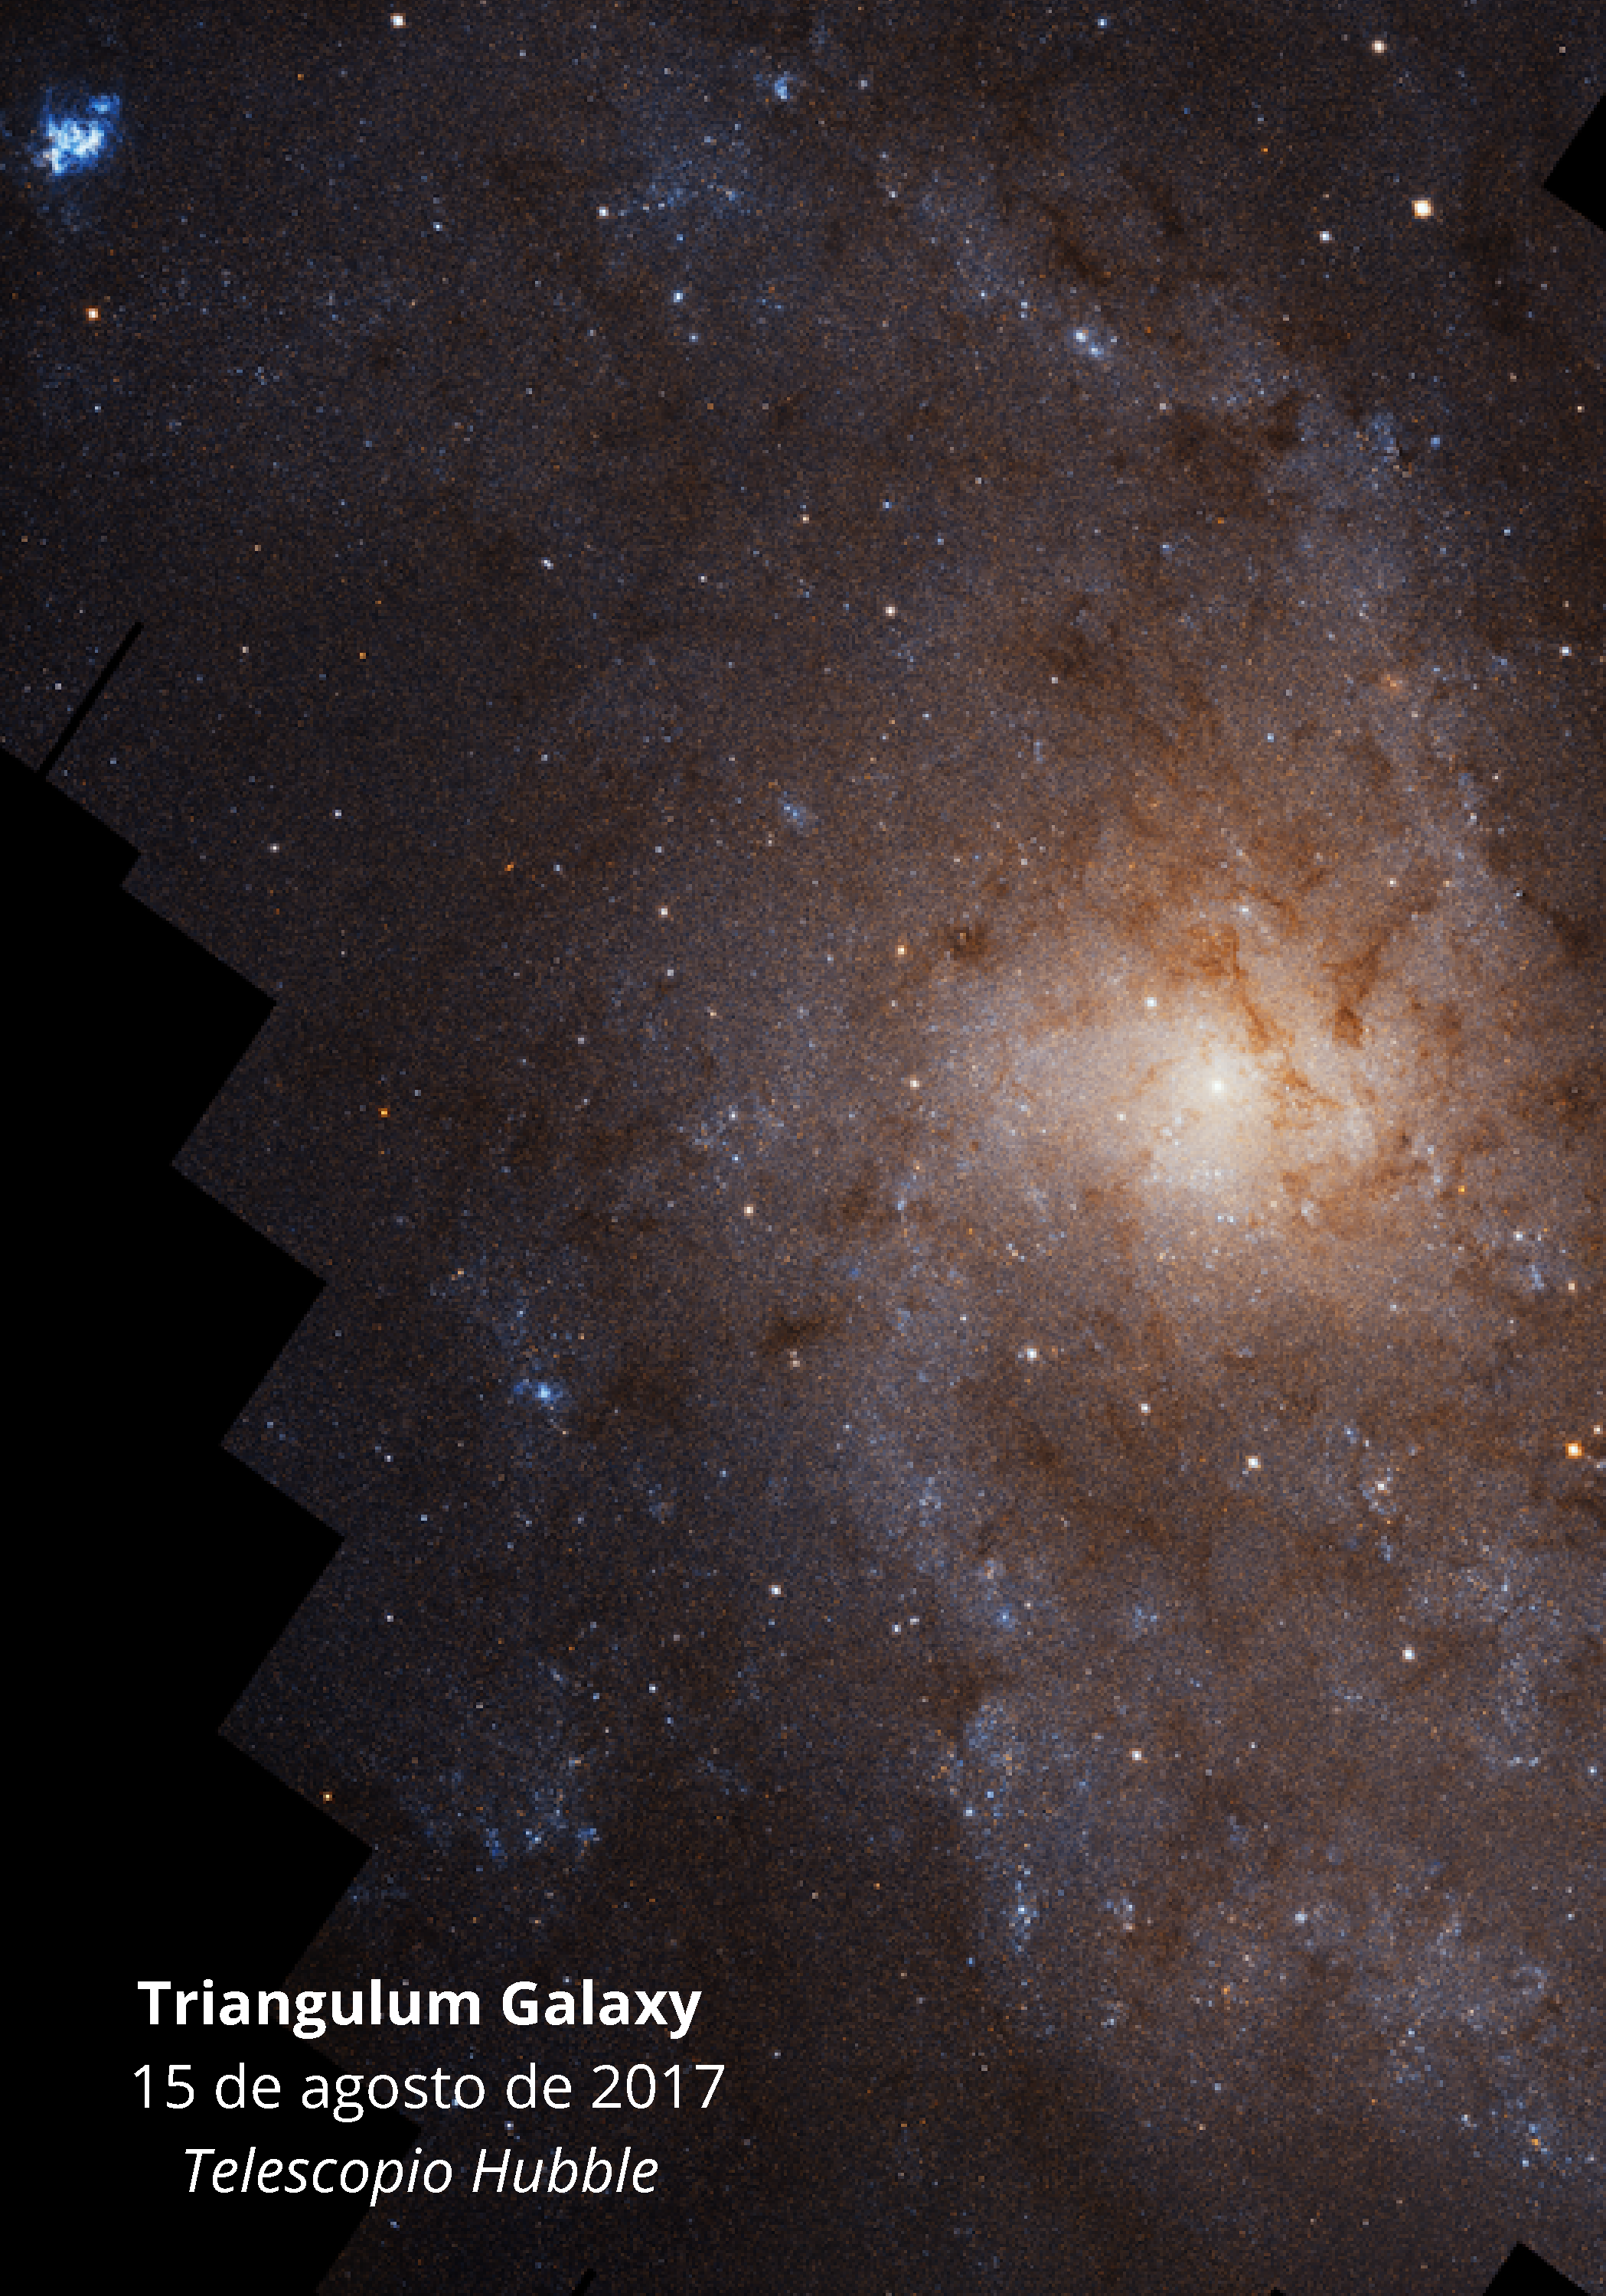
\includegraphics[width=\paperwidth]{Pictures/background.pdf}};
\draw (current page.center) node [fill=blue!30!white,fill opacity=0.6,text opacity=1,inner sep=1cm]{\Huge\centering\bfseries\sffamily\parbox[c][][t]{\paperwidth}{\centering Introducción a la astronomía\\[15pt] % Book title
{\Large Notas de clase}\\[20pt] % Subtitle
{\huge Rudik Roberto Rompich}}}; % Author name
\end{tikzpicture}
\vfill
\endgroup

%----------------------------------------------------------------------------------------
%	COPYRIGHT PAGE
%----------------------------------------------------------------------------------------

\newpage
~\vfill
\thispagestyle{empty}

\noindent Copyright \copyright\ 2020 Rudik Rompich\\ % Copyright notice

\noindent \textsc{Published by Rudiks}\\ % Publisher

\noindent \textsc{rudiks.com}\\ % URL

\noindent Licensed under the Creative Commons Attribution-NonCommercial 3.0 Unported License (the ``License''). You may not use this file except in compliance with the License. You may obtain a copy of the License at \url{http://creativecommons.org/licenses/by-nc/3.0}. Unless required by applicable law or agreed to in writing, software distributed under the License is distributed on an \textsc{``as is'' basis, without warranties or conditions of any kind}, either express or implied. See the License for the specific language governing permissions and limitations under the License.\\ % License information, replace this with your own license (if any)

\noindent \textit{First printing, October 2020} % Printing/edition date

%----------------------------------------------------------------------------------------
%	TABLE OF CONTENTS
%----------------------------------------------------------------------------------------

%\usechapterimagefalse % If you don't want to include a chapter image, use this to toggle images off - it can be enabled later with \usechapterimagetrue

\chapterimage{Pictures/0002} % Table of contents heading image

\pagestyle{empty} % Disable headers and footers for the following pages

\tableofcontents % Print the table of contents itself

\cleardoublepage % Forces the first chapter to start on an odd page so it's on the right side of the book

\pagestyle{fancy} % Enable headers and footers again

%----------------------------------------------------------------------------------------
%	PART
%----------------------------------------------------------------------------------------

\part{Elementales}

%----------------------------------------------------------------------------------------
%	CHAPTER 1
%----------------------------------------------------------------------------------------

\chapterimage{Pictures/0001} % Chapter heading image

\chapter{Elementales}

\section{Repaso}\index{Repaso}

\subsection{El Sistema Solar}

\subsubsection{El sol}
\begin{enumerate}
    \item El sol tiene 99,85 de la masa, 0.135 planetas, comentas,satélites..., 0.015 el resto...
    \item El sol es una estrella tipo G2, hidrógeno, helio y metales.
    \item El sol más brillante que el 83 por ciento de las estrellas en la galaxia. (Enanas rojas las más amplias). 
\end{enumerate}

\subsection{Los planetas}
    \begin{itemize}
        \item Orbitan el sol. 
        \item Masivos para ser esféricos; pero no lo suficiente para iniciar fusión nuclear. 
        \item No hay planetesimales.
        \item Planetas rocosos y gaseosos. 
        
    \end{itemize}
    
\begin{remark}
Tidal locking; la misma cara a un objeto que orbita
\end{remark}
\subsubsection{La Tierra}
\begin{itemize}
    \item La luna hace que la rotación de la tierra sea menor 
    \item Causa la inclinación de la tierra de 23.5 
\end{itemize}

\subsubsection{Otros planetas}
\begin{itemize}
    \item Júpiter: 4 sistemas de anillos, más tenues que los de Saturno. 
    \item Saturno: Menor densidad a la del agua. 
    \item Urano: eje de rotación paralelo al plano de la elíptica. 
    \item Neptuno: llueve diamantes
    
    
\end{itemize}

\subsection{La zona habitable}
\begin{itemize}
    \item Región en donde la existencia de agua. 
    \item Presión atmosférica 
    \item Campo magnético 
    
\end{itemize}

\subsection{Cinturón de asteroides}

\begin{itemize}
    \item Región entre Marte y Júpiter
    \item Cuerpos sólidos e irregulares. 
    \item Ceres (esférico), Vesta, Pallas, Hygie
\end{itemize}

\subsection{Cinturón de Kuiper}
\begin{itemize}
    \item Orbita de Neptuno hasta 55 AU 
    \item Asteroides y planetas enanos. 
    \item 20 ancho y 200 masivo comparado al cinturón de asteroides. 
    \item A los objetos se les llama transneptunianos. 
    \item Neptuno tiene un gran efecto 
\end{itemize}

\subsection{Planetas enanos}
\begin{itemize}
    \item No han limpiado su órbita de planetesimales.
\end{itemize}

\subsection{Cometas}
\begin{itemize}
    \item Cuerpo de hizo que emana gases cuando se caliente
    \item Outgassing 
\end{itemize}

\subsection{Material interplanetario}
\begin{itemize}
    \item Polvo 
    \item Piedra y hielo
    \item Meteoroide (<100) 
    \item Asteroide (>100) 
    \item Comentas
\end{itemize}

\subsection{Mete...}
\begin{itemize}
    \item Meteoroide (lalala) 
    \item Meteoro (entrando a orbita)
    \item Meteorito (estrellado) 

\end{itemize}

\subsection{Heliosfera}
\begin{itemize}
    \item Región influenciada por el viento solar y el campo magnético. 
    \item Protege de rayos cósmicos 
\end{itemize}

\subsection{Nube de Oort}
\begin{itemize}
    \item Después de la heliosfera, entre 2000 AU a 200,000 AU 
    \item Planetesimales de hielo 
    \item Límite del SS y esfera de Hill 
    
\end{itemize}

\subsection{Esfera de Hill}
\begin{itemize}
    \item Región en donde existe la atracción gravitatoria. 
\end{itemize}

\section{Propiedades del SS}
\begin{itemize}
    \item Planetas aislados
    \item Órbitas casi circulares
    \item Mismo plano 
    \item Diferenciado interior y exterior
    \item Asteroides viejos 
    \item Venus orbita en el sentido contrario 
    \item Rocosos: pequeños y densos. Grandes: gaseosos y enormes. 
    \item Todos los gaseosos tiene anillos. 
\end{itemize}

%----------------------------------------------------------------------------------------
%	CHAPTER 1
%----------------------------------------------------------------------------------------

\chapterimage{Pictures/0002} % Chapter heading image

\chapter{Formación del sistema solar}

\section{Formación del sistema solar}
\subsection{Teoría nebular}
\begin{itemize}
    \item Nube que se contrae
    \item Rota rápido, por el momento angular
    \item Fuerza centrípeta se opone a la contracción 
    \item Disco 
    \item \textbf{NO explica interno y externo}
    \item planetas no se forman en la nube
\end{itemize}

\subsection{Teoría de la condensación}
\begin{itemize}
    \item Teoría nebular pero con polvo interestelar 
    \item Polvo microscópico expulsado por supernovas.
    \item Partículas de hielo y roca 
\end{itemize}

\subsection{Polvo interestelar}
\begin{itemize}
    \item Polvo enfría materia
    \item Reduce la presión externa 
    \item Actúa como condensación, los átomos se adhieren a él.
    \item Acretan y acretan -> Planetesimales -> Protoplaneta -> Acreción
    \item \textbf{Fragmentación} Se escapó como asteroide o cometa.
\end{itemize}

\subsection{Diferenciación del SS}
\begin{itemize}
    \item Composición de un planeta depende de su posición. 
    \item Centro: partículas en moléculas y el polvo desapareció.
    \item Exteriores: el polvo se mantuvo igual. 
    \item El polvo se enfrío en todos lados menos en su centro. 
\end{itemize}

\begin{remark}
Planetas exteriores más representativos del universo.
\end{remark}

\begin{notation}
Teoría de condensación - acreción explica los planetas terrestres, pero no los gigantes. 
\end{notation}

\subsection{Teoría Núcleo-Acreción}
\begin{itemize}
    \item Rocosos: Sí hay acreción hasta llegar a protoplanetas. 
    \item SS exterior: menos temperatura, más materiales. Campo gravitatorio era grande para acretar grandes cantidades de gas. 
    \item Densas atmósferas. 
    \item \textbf{No hubo suficiente tiempo}
\end{itemize}

\subsection{Teoría de inestabilidad gravitacional}
\begin{itemize}
    \item Nebulosa no era uniforme, habían grumos. 
    \item Grumos colapsaron bajo su propia gravedad. 
    \item 4 grandes protoplanetas, acretaron gas y polvo rápidamente por su gran gravedad. 
\end{itemize}

\begin{remark}
\textbf{Núcleo-Acreción: } predice masas de \textbf{20M}\\
\textbf{Inestabilidad-gravitacional} predice masas de \textbf{6M}
\end{remark}

\begin{notation}
SS exterior: planetas actuaron como soles y lunas como plenetas\\
SS interior: planetesimales capturados. 
\end{notation}

\begin{remark}
\textbf{Migración de planetas gigantes}
Los planetas gigantes migraron lejos del sol y luego migraron hacia él.\\
\textbf{Dos posibilidades: }
\begin{itemize}
    \item Nebulosa solar más fría
    \item Júpiter se formó en el cinturón de Kuiper. 
\end{itemize}

\end{remark}

\subsection{Otras cosas nice...}
\begin{itemize}
    \item SS interior: planetesimales que no fueron capturados o acretados fueron expulsados más allá de la órbita de Marte. 
    \item Cinturón de asteroides: un planeta que no se formó por el fuerte campo gravitatorio de Júpiter. 
    \item Cinturón de Kuiper: planetesionales de Urano y Neptuno.  
    \item La nube de Oort: planetesimales de Urano/Neptuno expulsados hacia Saturno y Júpiter; para finalmente estos mandarlos lejos. 
    \item El agua de la tierra probablemente llegó de un cometa. 
\end{itemize}

\begin{figure}[h]
\centering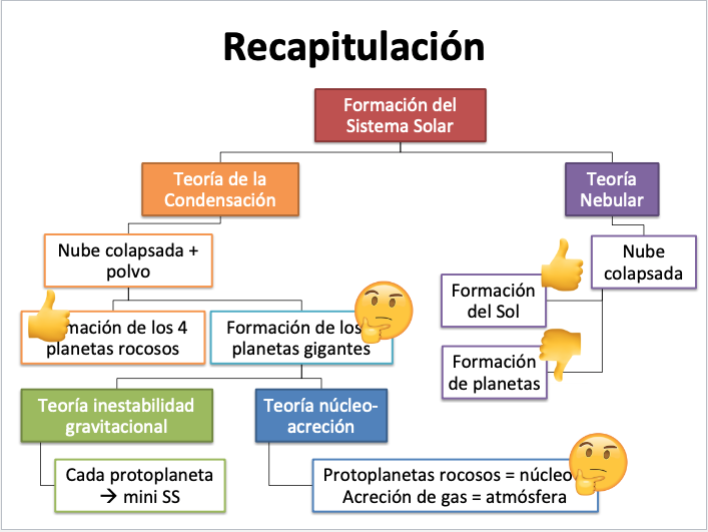
\includegraphics[scale=0.6]{Pictures/ss_formacion}
\caption{Formación del sistema solar}
\label{fig:placeholder} 
\end{figure}

\chapter{Otras formaciones específicas}
\section{Luna}

\subsection{La luna como tal...}
\begin{itemize}
    \item La luna no tiene un núcleo de Fe grande, masivo y denso como la tierra. 
    \item Deficiente en metales pesados comparado con la Tierra. 
    \item Núcleo sólido y no líquido
    \item Poroso -> Disminuye su densidad promedio. 
    \item Lado oscuro es más grueso que el lado que ve a la tierra. 
\end{itemize}

\subsection{Formación de la luna}

\subsubsection{Teoría de la hermana}
\begin{itemize}
    \item Luna y Tierra se formaron al mismo tiempo por planetesimales. 
    \item Sistema binario entre ambos. 
    \item Evolucionó a lo que es ahora. 
    \item \textbf{Problema: } Luna y Tierra distinta composición. 
\end{itemize}
\subsubsection{Teoría de la captura}
\begin{itemize}
    \item La luna se formó al mismo tiempo que la tierra, pero en otra \textbf{región}. 
    \item Luna pasó cerca de la Tierra y esta la capturó. 
    \item \textbf{Problema: }Luna es grande y los mantos de la Luna y Tierra son parecidos.
\end{itemize}
\subsubsection{Teoría de la hija}
\begin{itemize}
    \item Luna se formó de la Tierra misma. 
    \item Tierra giraba rápido y una parte del Océano Pacífico se desprendió. 
    \item \textbf{Problema: } No se explica como la Tierra giraba tan rápido y si la luna hubiera sido expulsada, la órbita no habría sido estable. 
\end{itemize}
\subsubsection{Teoría de la impacto}

\begin{itemize}
    \item \textbf{Más favorecida} Captura+Hija
    \item Un objeto del tamaño de Marte colisionó con la Tierra. 
    \item El objeto resultado se acretó formando la Luna. 
    \item Explica que la Tierra y la luna tengan un \textbf{manto} similar. 
    \item El núcleo de Fe del objeto quedó en la Tierra. 
    \item \textbf{Únicamente a la Tierra}
\end{itemize}

\section{La Tierra}

\subsection{La atmósfera}
\subsubsection{Atmósfera primaria}
\begin{itemize}
    \item Hidrógeno -> Helio -> Metano -> Metano -> Amoniaco -> Vapor de agua 
\end{itemize}
\subsubsection{Atmósfera secundaria}
\begin{itemize}
    \item Expulsada del interior de la Tierra. 
    \item Actividad volcánica. 
    \item Radiación del sol: dividió los componente ricos en hidrógeno.
    \item Temperatura bajó, el vapor de agua se condensó y formó los océanos. 
    \item El $O_2$ apareció por los organismos biológicos. 
    \item El $El O_3$ protege de los rayos UV.
\end{itemize}

\subsection{El cielo}
\begin{itemize}
    \item El cielo es azul debido a la dispersión de Rayleigh.
\end{itemize}

\begin{remark}
En Marte se comporta distinto la atmósfera
\begin{itemize}
    \item Por la dispersión de Mie
    \item Dispersión de la luz por polvo 
    \item Rojas se ven beneficiadas. 
    \item Depende del ángulo de incidencia. 
\end{itemize}
\end{remark}

\chapter{Exo-Sistemas Solares}
\section{Exo-Sistemas Solares}
Hasta ahora sabemos de la teoría de la condensación: 
\begin{itemize}
    \item La teoría de la condensación explica la estructura del SS.
    \item Flexible. Explica otras situaciones: nuestra Luna, la rotación lenta de Venus y la rotación en el sentido contrario de Venus. 
\end{itemize}

\subsection{Detección de planetas}
Indirectas
\begin{itemize}
    \item Se observa a la estrella anfitriona
    \item \textbf{Variaciones de la velocidad radial}
    \item \textbf{Tránsitos planetarios}
\end{itemize}
Directas
\begin{itemize}
    \item Luz de la estrella per se. 
\end{itemize}

\subsubsection{Indirectas}
\textbf{Velocidad radial}
\begin{itemize}
    \item Sistemas binarios (planeta+estrella). 
    \item Solo se da un límite inferior a la masa del planeta. 
    \item Es necesaria la inclinación del sistema.
\end{itemize}
\begin{remark}
The radial velocity of an object with respect to a given point is the rate of change of the distance between the object and the point. That is, the radial velocity is the component of the object's velocity that points in the direction of the radius connecting the point and the object. In astronomy, the point is usually taken to be the observer on Earth, so the radial velocity then denotes the speed with which the object moves away from the Earth (or approaches it, for a negative radial velocity).
\end{remark}
\textbf{Tránsitos}
\begin{itemize}
    \item Tamaño relativo del planeta respecto a la estrella.
    \item Qué tanto disminuyó la luz. 
\end{itemize}

\subsubsection{Directas}
\textbf{Imágenes del planeta}
\begin{itemize}
    \item Sustraer la luz de la estrella. 
    \item Observaciones con mucha resolución angular y mucho constaste.
    \item Únicamente planetas grandes y brillantes.
    \item Lejos de su estrella. 
    \item Se detectan: Temperatura, Radio, Masa y Atmósfera
\end{itemize}


\begin{figure}[h]
\centering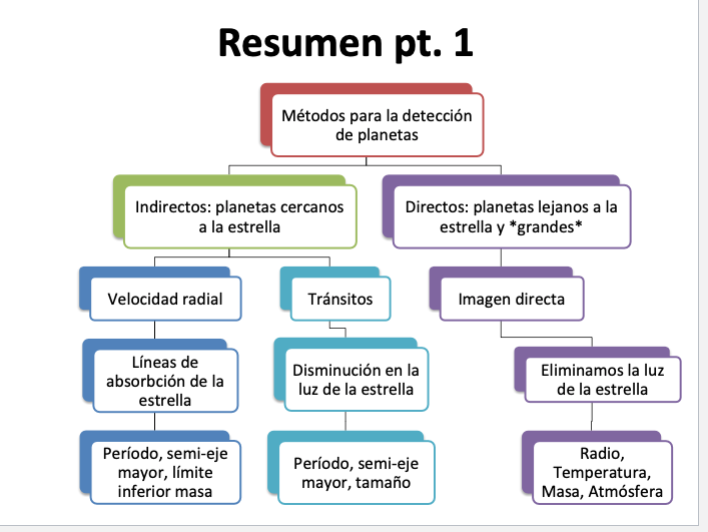
\includegraphics[scale=0.6]{Pictures/exo.png}
\caption{Formación del sistema solar}
\label{fig:placeholder} 
\end{figure}

%----------------------------------------------------------------------------------------
%	INDEX
%----------------------------------------------------------------------------------------

\cleardoublepage % Make sure the index starts on an odd (right side) page
\phantomsection
\setlength{\columnsep}{0.75cm} % Space between the 2 columns of the index
\addcontentsline{toc}{chapter}{\textcolor{blue}{Index}} % Add an Index heading to the table of contents
\printindex % Output the index

%----------------------------------------------------------------------------------------

\end{document}
